\documentclass{beamer}
\makeatletter
\renewcommand*\env@matrix[1][*\c@MaxMatrixCols c]{%
	\hskip -\arraycolsep
	\let\@ifnextchar\new@ifnextchar
	\array{#1}}
\makeatother
%%\usepackage[style=verbose,backend=biber]{biblatex}
%%\addbibresource{ref.bib}
\setbeamerfont{footnote}{size=\tiny}
\beamertemplatenavigationsymbolsempty
% THEMES
% http://deic.uab.es/~iblanes/beamer_gallery/index_by_theme.html
% You can uncomment the themes below if you would like to use a different
% one:
%\usetheme{AnnArbor}
%\usetheme{Antibes}
%\usetheme{Bergen}
%\usetheme{Berkeley}
%\usetheme{Berlin}
\usetheme{Boadilla}
%\usetheme{boxes}
%\usepackage{figure}
%\usetheme{CambridgeUS}
%\usetheme{Copenhagen}
%\usetheme{Darmstadt}
%\usetheme{default}
%\usetheme{Frankfurt}
%\usetheme{Goettingen}
%\usetheme{Hannover}
%\usetheme{Ilmenau}
%\usetheme{JuanLesPins}
%\usetheme{Luebeck}
%\usetheme{Madrid}
%\usetheme{Malmoe}
%\usetheme{Marburg}
%\usetheme{Montpellier}
%\usetheme{PaloAlto}
%\usetheme{Pittsburgh}
%\usetheme{Rochester}
%\usetheme{Singapore}
%\usetheme{Szeged}
%\usetheme{Warsaw}

%PACKAGES
\usepackage{color}
\usepackage{tikz}
\usepackage{caption}
\usepackage{graphicx}
\usepackage{amsmath}
\usepackage{amssymb}
\usepackage{natbib}
\usepackage[utf8]{inputenc}
\usepackage{pgf}
\usepackage{tikz} %Use Tiks to plot graph
\usetikzlibrary{arrows,automata}
%figure package
\usepackage{float}


%START PRESENTATION DETAILS
\title{}

\DeclareMathOperator*{\argmin}{argmin}
\DeclareMathOperator{\E}{\mathbb{E}}
% correct bad hyphenation here
\hyphenation{op-tical net-works semi-conduc-tor}




% A subtitle is optional and this may be deleted
%\subtitle{}

\author{Alok Deshpande}
% - Give the names in the same order as the appear in the paper.
% - Use the \inst{?} command only if the authors have different
%   affiliation.

% \institute[University of Toronto] % (optional, but mostly needed)
% {
%   \inst{1}%
%   Department of Electrical and Computer Engineering\\
%   University of Toronto
%   \and
%   \inst{2}%
%   Department of Theoretical Philosophy\\
%   University of Elsewhere}
% - Use the \inst command only if there are several affiliations.
% - Keep it simple, no one is interested in your street address.

\date{February 7, 2017}
% - Either use conference name or its abbreviation.
% - Not really informative to the audience, more for people (including
%   yourself) who are reading the slides online

%\subject{}
% This is only inserted into the PDF information catalog. Can be left
% out. 

% If you have a file called "university-logo-filename.xxx", where xxx
% is a graphic format that can be processed by latex or pdflatex,
% resp., then you can add a logo as follows:

% \pgfdeclareimage[height=0.5cm]{university-logo}{university-logo-filename}
% \logo{\pgfuseimage{university-logo}}

% Delete this, if you do not want the table of contents to pop up at
% the beginning of each subsection:
% \AtBeginSubsection[]
% {
%   \begin{frame}<beamer>{Outline}
%     \tableofcontents[currentsection,currentsubsection]
%   \end{frame}
% }


%START PRESENTATION
\begin{document}
	
	\begin{frame}
	\titlepage
\end{frame}

%Manual outline
%\begin{frame}{Outline}
%\begin{itemize}
%	\item System and Attack Model
%	\item Undetectable Attack, Unidentifiable Attack, {\color{red}Structurally Undetectable Attack}
%	\item An Example Related to My Current Work
%	\item Monitoring Design
%\end{itemize}
%\end{frame}
%--------------------- vs --------------------------
%AUTOMATED outline
\begin{frame}{Outline}
\tableofcontents
% You might wish to add the option [pausesections]
\end{frame}
% Section and subsections will appear in the presentation overview
% and table of contents.

\section{Background}
\begin{frame}{Background}
	\begin{itemize}
		\item Battery life is critical to EV operation (e.g. driving time)
		\item Common design choice is hybrid power supply %%%/footcite{Paper 1}
		\subitem typically battery and supercapacitor
		\subitem improves battery life
		\item Reason: each is best suited for specific energy demand (load) profile %%%/footcite{Paper 1}}
		\subitem Supercapacitor: high power output; limited energy capacity
		\subitem Battery: opposite
	\end{itemize}
\end{frame}
\begin{frame}{Problem}
	\begin{itemize}
		\item Goal: optimal sequence of energy discharges from each storage
		\item Requirements:
		\subitem Constraint: net discharge = random demand
		\subitem Minimize: power transfer costs for each storage device
		\subitem Minimize: unnecessary energy transfers (losses)
	\end{itemize}
\end{frame}

\section{Model}

\begin{frame}{Definitions and Constraints}
\begin{itemize}
	\item Have separate charging and discharging (most general)
	\item Account for differing levels of leakage from each storage
	\item Indices\\
	$t$: discrete time step index\\
	$j$: storage device number (1: battery, 2: supercapacitor)\\
	\item Parameters\\
	$\alpha^{C}$: charging efficiency\\
	$\alpha^{D}$: discharging efficiency\\
	$\beta$: storage efficiency factor (constant)\\
	$N$: number of steps (DP horizon)\\
	$K$: cost weighting factor for rate (relative to cost of energy loss)\\
	\item Variables\\
	$L$: load energy demand (random)\\
	$E$: energy state of storage device\\
	$D$: energy released by discharging (AFTER loss)\\
	$C$: energy consumed by charging (BEFORE loss)\\
	$J$: cost function
	
	\item Supply-demand balance: 
	\begin{equation} \label{eq:BalanceEqn}\left[D_{1}(t)\right] + \left[D_{2}(t) - C_{2}(t)\right] = L(t) \end{equation}
	
	\item Bounds on stored energy: 
	\begin{equation}E_{j}^{min}\leq E_{j}(t)\leq E_{j}^{max}\end{equation}
	\item Bounds on charging:
	\begin{equation}0\leq C_{2}(t)\leq C_{2}^{max}\end{equation}
	\item Bounds on discharging:
	\begin{equation}0\leq D_{j}(t)\leq D_{j}^{max}\end{equation}
\end{itemize}
\end{frame}

\begin{frame}{Recursive State Equations}
\begin{itemize}
	\item Based on common formulation for a single storage %%%/footcite{Paper 3}
	\item Battery can only supply load or supercapacitor (no charging):
	\begin{equation}\label{eq:StateEq1}E_{1}(t+1)=\beta_{1}E_{1}(t)+\left[-\frac{1}{\alpha_{1}^{D}}D_{1}(t)\right] \end{equation}
	\item Supercapacitor can only supply load, but can be charged by battery:
	\begin{equation}\label{eq:DPStateEq2}E_{2}(t+1)=\beta_{2}E_{2}(t)+\left[\alpha_{2}^{C}[D_{1}(t)+D_{2}(t)-L(t)]-\frac{1}{\alpha_{2}^{D}}D_{2}(t)\right]\end{equation}
	\item PICTURE GOES HERE
	\includegraphics[width=4in, height=3in]{fault.eps}
\end{itemize}
\end{frame}

\begin{frame}{Cost Function}
\begin{itemize}
	 \item Minimize discharge rate
	 for the first storage device (battery):
	 \begin{equation}J_{rate}=min\left[\sum_{i=0}^{N}K\left[D_{1}(t)\right]^{2}\right]\end{equation}
	 \subitem Quadratic cost in time penalizes more for high excursions
 	 \subitem As done in many %%%/footcite{Hybrid Storage MPC}
 	 \subitem Alternatives:
 	 \subsubitem Linear in time (very simplistic) %%%/footcite{An LP approach…} %%%/footcite{StorageSizeMartinez}
 	 \subsubitem Arbitrarily convex in cycle-domain (too complex) %%%/footcite{Cyclic demand}
 	 
	 \item Minimize power loss due to energy transfers
	 \begin{equation}J_{loss}=\mathop{\E}_{L(t)} \Biggl\{min\left[\sum_{i=0}^{N}
	 (1-\alpha_{1}^{D})D_{1}(t)+
	 (1-\alpha_{2}^{C})[D_{1}(t)+D_{2}(t)-L(t)]+
	 (1-\alpha_{2}^{D})D_{2}(t)
	 \right]\Biggr\}\end{equation}
	 \subitem Has "natural" loss weightings
	 
	 \item Combined cost function
	 \begin{equation}J=\mathop{\E}_{\substack{ L(t) \\ \forall t\in{1\dots N} }} \Biggl\{min\left[\sum_{i=0}^{N}K\left[D_{1}(t)\right]^{2} + (1-\alpha_{1}^{D})D_{1}(t)+
	 (1-\alpha_{2}^{C})[D_{1}(t)+D_{2}(t)-L(t)]+
	 (1-\alpha_{2}^{D})D_{2}(t)\right]\Biggr\}\end{equation}
	 
	 This is of the form:
	 \begin{equation}J=\mathop{\E}_{w(t)} \Biggl\{\min_{u}\left[\sum_{i=0}^{N}g(x(t),u(t),w(t))\right]\Biggr\}\end{equation}
	 for state $x(t)$, control $u(t)$ and random perturbation $w(t)$. Here, $g(\cdot)$ is the stage cost.
\end{itemize}
\end{frame}

\begin{frame}{Finite Horizon DP}
\end{frame}

\section{Finite Horizon DP Solution}
\begin{frame}{Bellman Equation formulation}
\begin{itemize}
	\item Can apply dynamic programming to find sequence of optimal controls ($u*(t)$)
	\item Reformulate as Bellman’s equation:
	\begin{multline}
	J_{t}[x(t),w(t)]=\min_{u} g(x(t),u(t),w(t)) + \mathop{\E}_{w(t+1)} \{J_{t+1}[f(x(t),u(t),w(t)),w(t+1)]\}
	\end{multline}
	so, can solve recursively for N iterations %%%/footcite{Bertzekas??}
	\item In this case:
	\begin{multline}
	J_{t}[E_{1}(t),E_{2}(t),L(t)] = \min_{D_{1},D_{2}}
	(1-\alpha_{1}^{D})D_{1}(t) 
	+ K[D_{1}(t)]^{2}\\
	+(1-\alpha_{2}^{D})[D_{2}(t)]	  +(1-\alpha_{2}^{C})[D_{1}(t)+D_{2}(t)-L(t)]\\
	+\mathop{\E}_{L(t+1)}\{J_{t+1}[f_{1}(E_{1}(t),D_{1}(t)), f_{2}(E_{2}(t),D_{1}(t),D_{2}(t),L(t)), L(t+1)]\}
	\end{multline}
\end{itemize}
\end{frame}

\begin{frame}{Solution}
\begin{itemize}
	\item Choose terminal cost of 0
	\subitem assume vehicle reaches destination
	\subitem hence, assume not fully discharged in <N stages
	\item Then, costs are $\cdots$
	\subitem $N^{th}$ stage:
	\begin{equation}
	J_{N}[x(N),w(N)]=0
	\end{equation}		
	\subitem $(N-1)^{th}$ stage: \\
	\begin{multline}
	J_{N-1}[x(N-1),w(N-1)]=\min_{u} g(x(N-1),u(N-1),w(N-1))+ \mathop{\E}_{w(N)}\{0\}
	\end{multline}
	\subitem Initial stage: \\	
	\begin{multline}
	J=J_{0}[x(0),w(0)]=\min_{u} g(x(0),u(0),w(0))\\
	+\left[\sum_{t=0}^{N-1}\mathop{\E}_{w(t)} \{
	g( f(x(t),u(t),w(t)) ,u(t+1),w(t+1))
	\}\right]
	\end{multline}
	where $f(\cdot)$ is the general recursive state equation
\end{itemize}
\end{frame}


\section{Example}
\begin{frame}{A Numerical Example}
\begin{itemize}
\item{Define the following\\
$A=\begin{bmatrix}[c c c c c c]
0  & 0  & 0  & 1  & 0  & 0 \\
0  & 0  & 0  & 0  & 1  & 0 \\
0  & 0  & 0  & 0  & 0  & 1 \\
-2 & 1  & 0  & 0  & 0  & 0 \\
1  & -2 & 1  & 0  & 0  & 0 \\
0  & 1  & -2 & 0  & 0  & 0 \\
\end{bmatrix}$,
$B_K=\begin{bmatrix}[c c]
0  & 0  \\
1  & 0  \\
0  & 0  \\
0  & 0  \\
0  & 1  \\
0  & 0  \\
\end{bmatrix}$,
$C=\begin{bmatrix}[c c c c c c]
1  & 0  & 0  & 0  & 0  & 0 \\
0  & 0  & 0  & 4  & 0  & 0 
\end{bmatrix}$, $B=I$, $E=I$.}
\item {Goal: To design $F$ and make the attack set $K$ structurally detectable with the closed loop system $A+BF$, {\color{red}from output $y$}}.
\end{itemize}
\end{frame}
\begin{frame}{A Numerical Example}
\begin{itemize}
\item After some numerical operation, I get
$A+BF=\begin{bmatrix}[c c c c c c]
-1.0573  & 0.45130  & 0  & 1  & 0  & 0 \\
0  & 0  & 0  & 0  & 1  & 0 \\
0  & 0  & 0  & 0  & 0  & 1 \\
-2 & 1  & 0  & 0  & -2.769  & 0 \\
1  & -2 & 1  & 0  & 0  & 0 \\
0  & 1  & -2 & 0  & 0  & 0 \\
\end{bmatrix}$
\end{itemize}
\end{frame}
\begin{frame}{A Numerical Example}
\begin{figure}[!htb]\centering
\begin{minipage}{0.49\linewidth}
\scalebox{0.6}{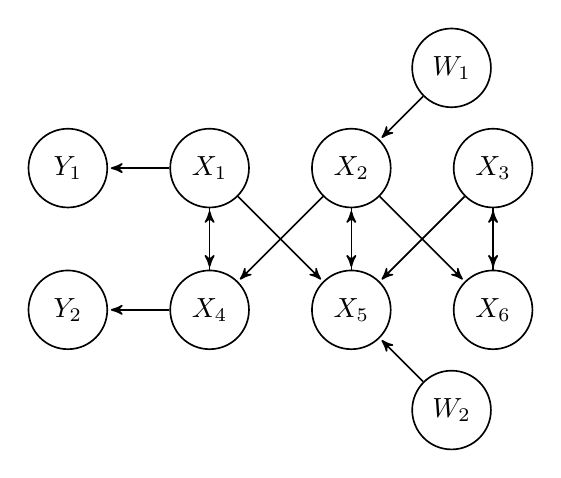
\begin{tikzpicture}[->,>=stealth',shorten >=1pt,node distance=1.8cm, semithick]
\tikzstyle{every state}=[fill=none,draw=black,text=black,minimum size=1cm]

\node[state]         (X1)                    {$X_1$};
\node[state]         (X2) [right of=X1]      {$X_2$};
\node[state]         (X3) [right of=X2]      {$X_3$};
\node[state]         (X4) [below of=X1]       {$X_4$};
\node[state]         (X5) [below of=X2]       {$X_5$};
\node[state]         (X6) [below of=X3]       {$X_6$};
\node[state]         (Y1) [left of=X1]       {$Y_1$};
\node[state]         (Y2) [left of=X4]       {$Y_2$};
\node[state]         (W1) [above right of=X2] {$W_1$};
\node[state]         (W2) [below right of=X5] {$W_2$};
\path (X1) edge              node {} (X4)
edge              node {} (X5)
edge              node {} (Y1)
(X2) edge              node {} (X4)
edge              node {} (X6)
edge              node {} (X5)
(X3) edge              node {} (X5)
edge              node {} (X6)
(X4) edge              node {} (X1)
edge              node {} (Y2)
(X5) edge              node {} (X2)
(X6) edge              node {} (X3)
(W1) edge              node {} (X2)
(W2) edge              node {} (X5);
\end{tikzpicture}}
\caption{Graph Representation of the Open-Loop Six Nodes Network, Only One Disjoint Path}
\end{minipage}
\begin {minipage}{0.49\linewidth}
\scalebox{0.6}{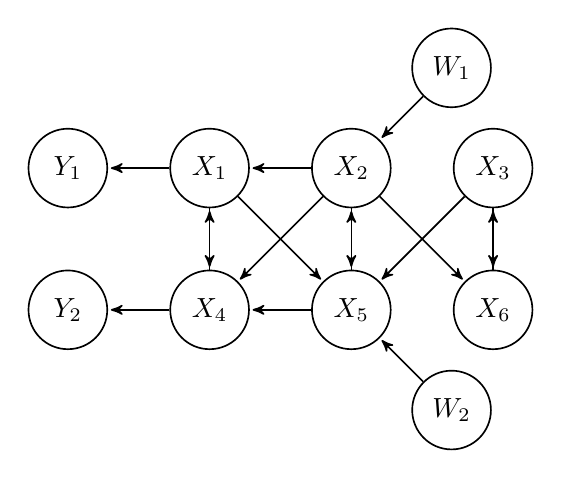
\begin{tikzpicture}[->,>=stealth',shorten >=1pt,node distance=1.8cm, semithick]
\tikzstyle{every state}=[fill=none,draw=black,text=black,minimum size=1cm]

\node[state]         (X1)                    {$X_1$};
\node[state]         (X2) [right of=X1]      {$X_2$};
\node[state]         (X3) [right of=X2]      {$X_3$};
\node[state]         (X4) [below of=X1]       {$X_4$};
\node[state]         (X5) [below of=X2]       {$X_5$};
\node[state]         (X6) [below of=X3]       {$X_6$};
\node[state]         (Y1) [left of=X1]       {$Y_1$};
\node[state]         (Y2) [left of=X4]       {$Y_2$};
\node[state]         (W1) [above right of=X2] {$W_1$};
\node[state]         (W2) [below right of=X5] {$W_2$};
\path (X1) edge              node {} (X4)
edge              node {} (X5)
edge              node {} (Y1)
(X2) edge              node {} (X4)
edge              node {} (X6)
edge              node {} (X5)
edge              node {} (X1)
(X3) edge              node {} (X5)
edge              node {} (X6)
(X4) edge              node {} (X1)
edge              node {} (Y2)
(X5) edge              node {} (X2)
edge              node {} (X4)
(X6) edge              node {} (X3)
(W1) edge              node {} (X2)
(W2) edge              node {} (X5);
\end{tikzpicture}}
\caption{Graph Representation of the Closed-Loop Six Nodes Network, Two Disjoint Paths}
\end{minipage}
\end{figure}
\end{frame}



\begin{frame}{A Numerical Example}
\begin{itemize}
\item From the open-loop transfer matrix, we notice that if making the attack
$\begin{bmatrix}[c]
u_1\\
u_2
\end{bmatrix}=
\begin{bmatrix}[c]
-\frac{1}{s}\\
1
\end{bmatrix}
U(s)$, then the attack cannot be detected from $y$.
\item Specifically, I made $u_1(t)=-10-10cos(t)$, $u_2(t)=sin(t)$. Let's see the simulation results.

\end{itemize}
\end{frame}
\begin{frame}{A Numerical Example}
\includegraphics[width=4in, height=3in]{fault.eps}
\end{frame}


\section{Monitor Design}
\begin{frame}{Monitor Design}

If the following holds, 
\begin{itemize}
\item $w(0)=x(0)$... {\color{red} if not, asymptotically converging}
\item $(E, A_D+GC)$ is regular and Hurwitz {\color{blue} modified, $A_D=\text{blkdiag}(A_1, A_2, ...A_N)$}
\item Must know all regular control input ...{\color{red} assume zero in the paper}
\item $(E_i,A_i,C_i)$ must be observable...{\color{red}this is very hard to guarantee} {\color{blue} modified}
\item $(E_i,A_i)$ is regular.. {\color{blue} modified}
\item $|sE-A|$ does not vanish for all $s$
\item the initial condition x(0) is consistent ... {\color{red}satisfy the algebraic equation, $Ax(0)+Bu(0)\in Im(E)$}
\item the unknown attack $u_K(t)$ is sufficiently smooth ... {\color{red} in case of impulsive input}
\item $\rho((j\omega E-A_D-GC)^-1A_C)<1$ for all $\omega \in R$ ... {\color{blue} extra}
\item All attacks are detectable
\end{itemize}
Then $r(t) = 0$ if and only if $u(t) = 0 $.
\end{frame}

\begin{frame}{Monitor Design}

How to do?%%/footcite{dorfler2013continuous}
\begin{itemize}
\item collect samples of $y_i(t), \forall i$.
\item set an initial stage $w_i(t) \forall i$.
\item set $k:=k+1$, compute $w_i^{(k)}(t)$, $t\in[0,T]$, by integrating\\
$E_i \dot{w}_i^{(k)}(t) = (A_i+G_iC_i)w_i^{(k)}(t) + \sum_{j\neq i}A_{ij}w_j^{(k-1)}(t)- G_iy_i(t)$.
\item transmit $w_i^{(k)}(t)$ to control center $j$ if $A_{ij}\neq 0$.
\item update $w_j^{(k)}(t)$ with signal received from control center $j$.
\end{itemize}
For sufficient large $k$, all $r_i(t)$ will goes to zero if there is no attack.
This is just in horizon $[0,T]$, we can have more time horizon.$[T,2T],....$.
\end{frame}

\end{document}